\subsection{Bell 412}
\begin{wrapfigure}{L}{0.5\textwidth}
  \begin{center}
    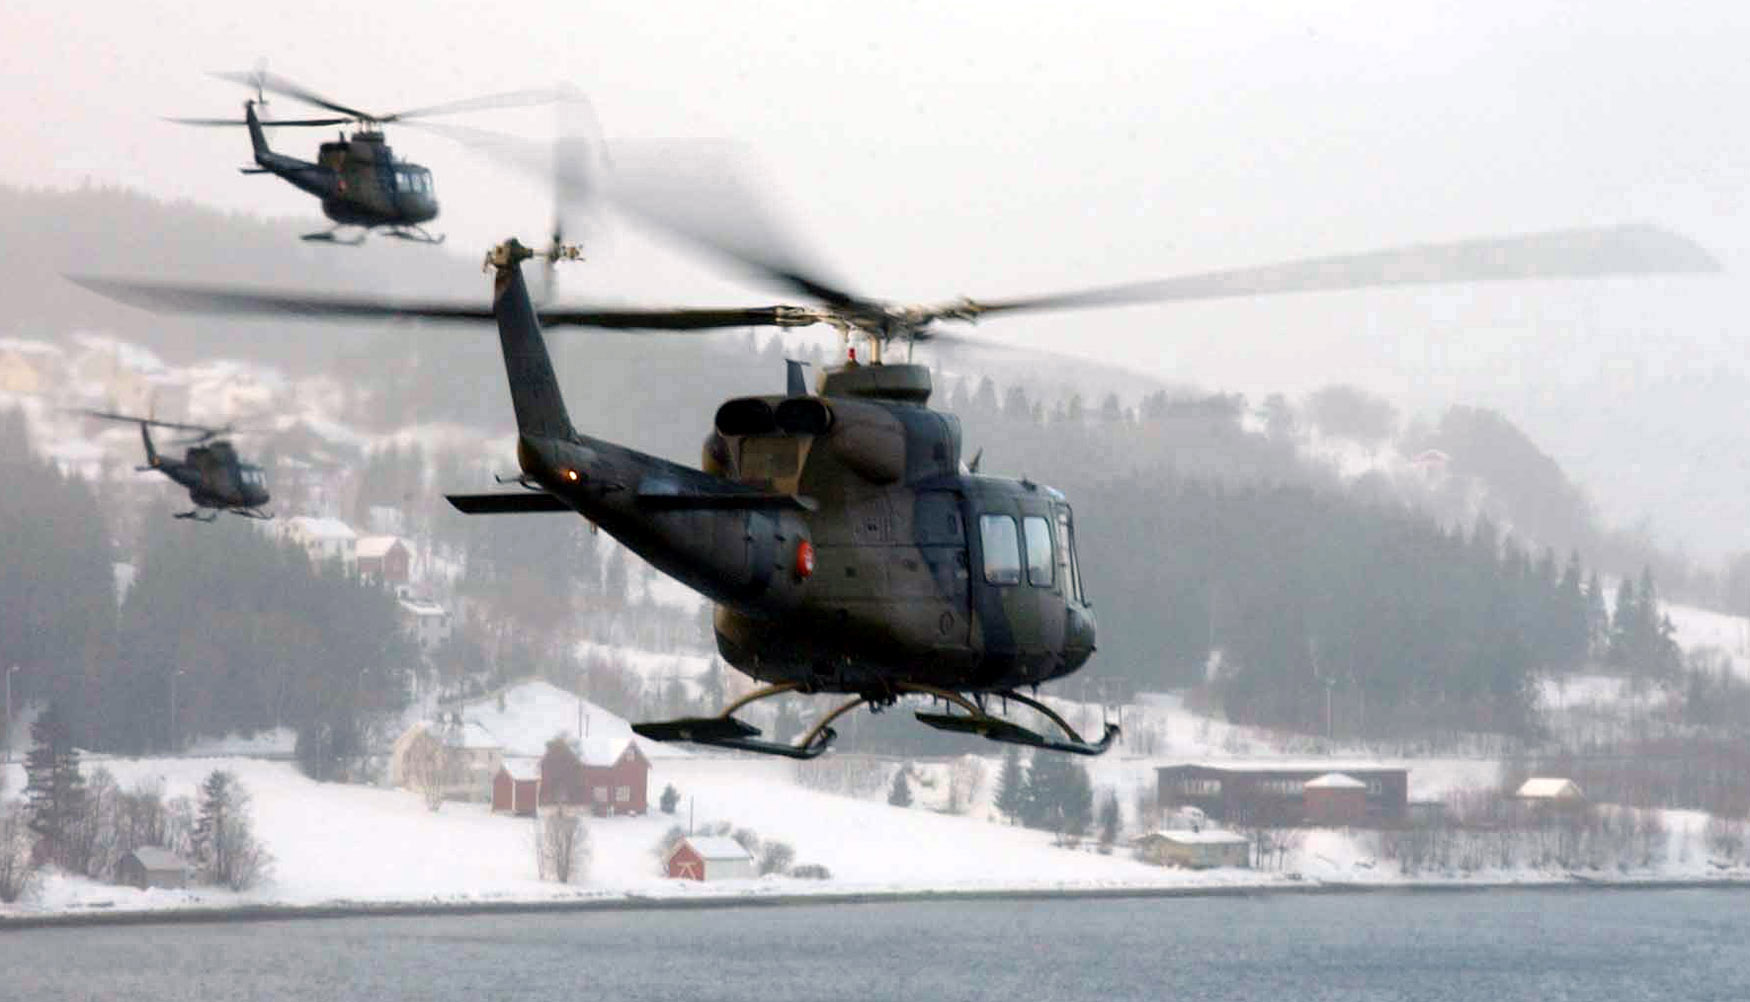
\includegraphics[width=0.40\textwidth]{images/bell.jpg}
  \end{center}
  \caption{Ejemplo de imagen a la izquierda}
\end{wrapfigure}
El Bell 412 es un helicóptero utilitario bimotor construido por Bell Helicopter Textron. Fue desarrollado a partir del modelo Bell 212. La mayor diferencia entre ambos es que el modelo 412 tiene cuatro palas en el rotor principal y el modelo 212 tiene solo dos. 
\subsubsection{Desarrollo}
El desarrollo se inició a finales de la década de los 70 cuando dos Bell 212 fueron convertidos en prototipos del 412. Se reemplazó el rotor de dos palas de los 212 por un avanzado rotor de cuatro palas con menor diámetro. Cada pala está construida con fibra de vidrio con estructura en panal de abeja tipo Nomex, y dispone de una banda de titanio resistente a la abrasión en el borde de ataque y una red pararrayos incluida en la estructura. La cabeza del rotor, también de nuevo diseño, está construida en una estructura de acero y aleación ligera, y dispone de cojinetes y amortiguadores elastoméricos.

Uno de los prototipos del Bell 412 voló por primera vez en agosto de 1979. El modelo inicial fue certificado en enero de 1981, mes en el que también empezaron las primeras entregas.1​

El modelo 412 fue seguido por el 412SP (Special Performance) versión que tenía mayor capacidad de combustible, mayor peso al despegue y un arreglo de asientos con mayor capacidad. En 1991, el 412HP (High Performance) fue una variante que mejoró la transmisión, reemplazando así a la versión SP.1​ La versión actual de producción es la 412EP (Enhanced Performance), la cual está equipada con un sistema de control automático dual digital.

Se han construido más de 700 helicópteros del modelo 412 (incluyendo 260 fabricados por AgustaWestland).2​ 
